The model captures changes in social interactions over time through a dynamic age-specific mixing matrix. The following
sections describe how this matrix is defined and how it captures the different non-pharmaceutical interventions implemented
in the analysed countries, including school closures.

\paragraph{Reference mixing matrices}
We extracted country-specific contact matrices using the \textit{conmat} R package which derives social mixing matrices from 
contact survey data. These matrices provide the average numbers of contacts per day between different age groups, disaggregated by the following 
locations: home, school, work, other locations. 

The overall contact matrix (before adjustments for mobility changes) results from the summation of the four location-specific 
contact matrices: \(C_{0} = C_{H} + m_S C_{S} + C_{W} + C_{L}\), where \(C_{H}\), \(C_{S}\), \(C_{W}\) and \(C_{L}\) are the age-specific
contact matrices associated with households, schools, workplaces and other locations, respectively. Note that the school contribution $C_{S}$ is 
multiplied by the factor $m_S$ that is varied during model calibration (see Section \ref{calibration}), in order to include uncertainty around 
the relative contribution of school contacts to overall mixing.

\paragraph{Modifications of contact rates over time}
\label{time_var_mixing}
To capture mobility changes over time, the contributions of the matrices \(C_{S}\), \(C_{W}\) and \(C_{L}\) vary with time such that the input contact matrix can be written as:

\begin{equation}
\label{eq_mixing}
  C(t)= h(t)^{2}C_{H}+ s(t)^{2} m_S C_{S}+ w(t)^{2}C_{W}+l(t)^{2}C_{L}
\end{equation}

The modifying functions $h$ (for households), $s$ (for schools), $w$ (for work) and $l$ (for other-locations) are each squared to capture the effect of the mobility changes on 
both the infector and the infectee in any given interaction that could potentially result in transmission. 

\vspace{5pt}
\textbf{School closure/re-opening}

Reduced attendance at schools is represented through the function $s$, which represents the proportion of all school students 
currently attending on-site teaching. If schools are fully closed at time $t$, \(s(t)=0\) and \(C_{S}\) does not contribute to the overall 
mixing matrix \(C(t)\). 
The function $s$ is derived from the UNESCO database on school closures since the start of the COVID-19 pandemic (\textcolor{red}{ADD REF HERE}).
This database provides school opening status over time as a categorical variable taking the following values: ``Fully open'', ``Partially open'', ``Academic break'', ``Closed due to COVID-19''.
Table \ref{tab:unesco_categories} indicates how the different categorical values are converted into the numerical function $s$.

\begin{table}[ht]  
  \begin{center}
      \begin{tabular}{p{5cm} | p{5cm}}
          \hline
          \textbf{UNESCO category} & \textbf{Assumed proportion of students on-site ($s(t)$)} \\
          \hline
          Fully open & 100\% \\
          Partially open & 10-30\% \\
          Academic break & 0\% \\
          Closed due to COVID-19 & 0\% \\
          \hline
      \end{tabular}
    \end{center}
      \caption{Assumed percentage of students on-site for the different UNESCO school closure categories.}
      \label{tab:unesco_categories}
  \end{table}

We included uncertainty around the value associated with the partial closure category, as there is no quantitative data available to 
inform this parameter. The partial closure periods are likely to be periods where only a small fraction of students such as children of ``essential workers'' were 
attending school. We assume that between 10 and 30\% of students attended on-site learning during these periods.

To model the counterfactual ``no school closure'' scenario, we assume that the schools were ``Fully open'' during the
periods reported as ``Partially open'' or ``Closed due to COVID-19''.

Figure \ref{fig:unesco} summarises the UNESCO data on school closure for the analysed countries.

\begin{figure}[p]
  \begin{center}
  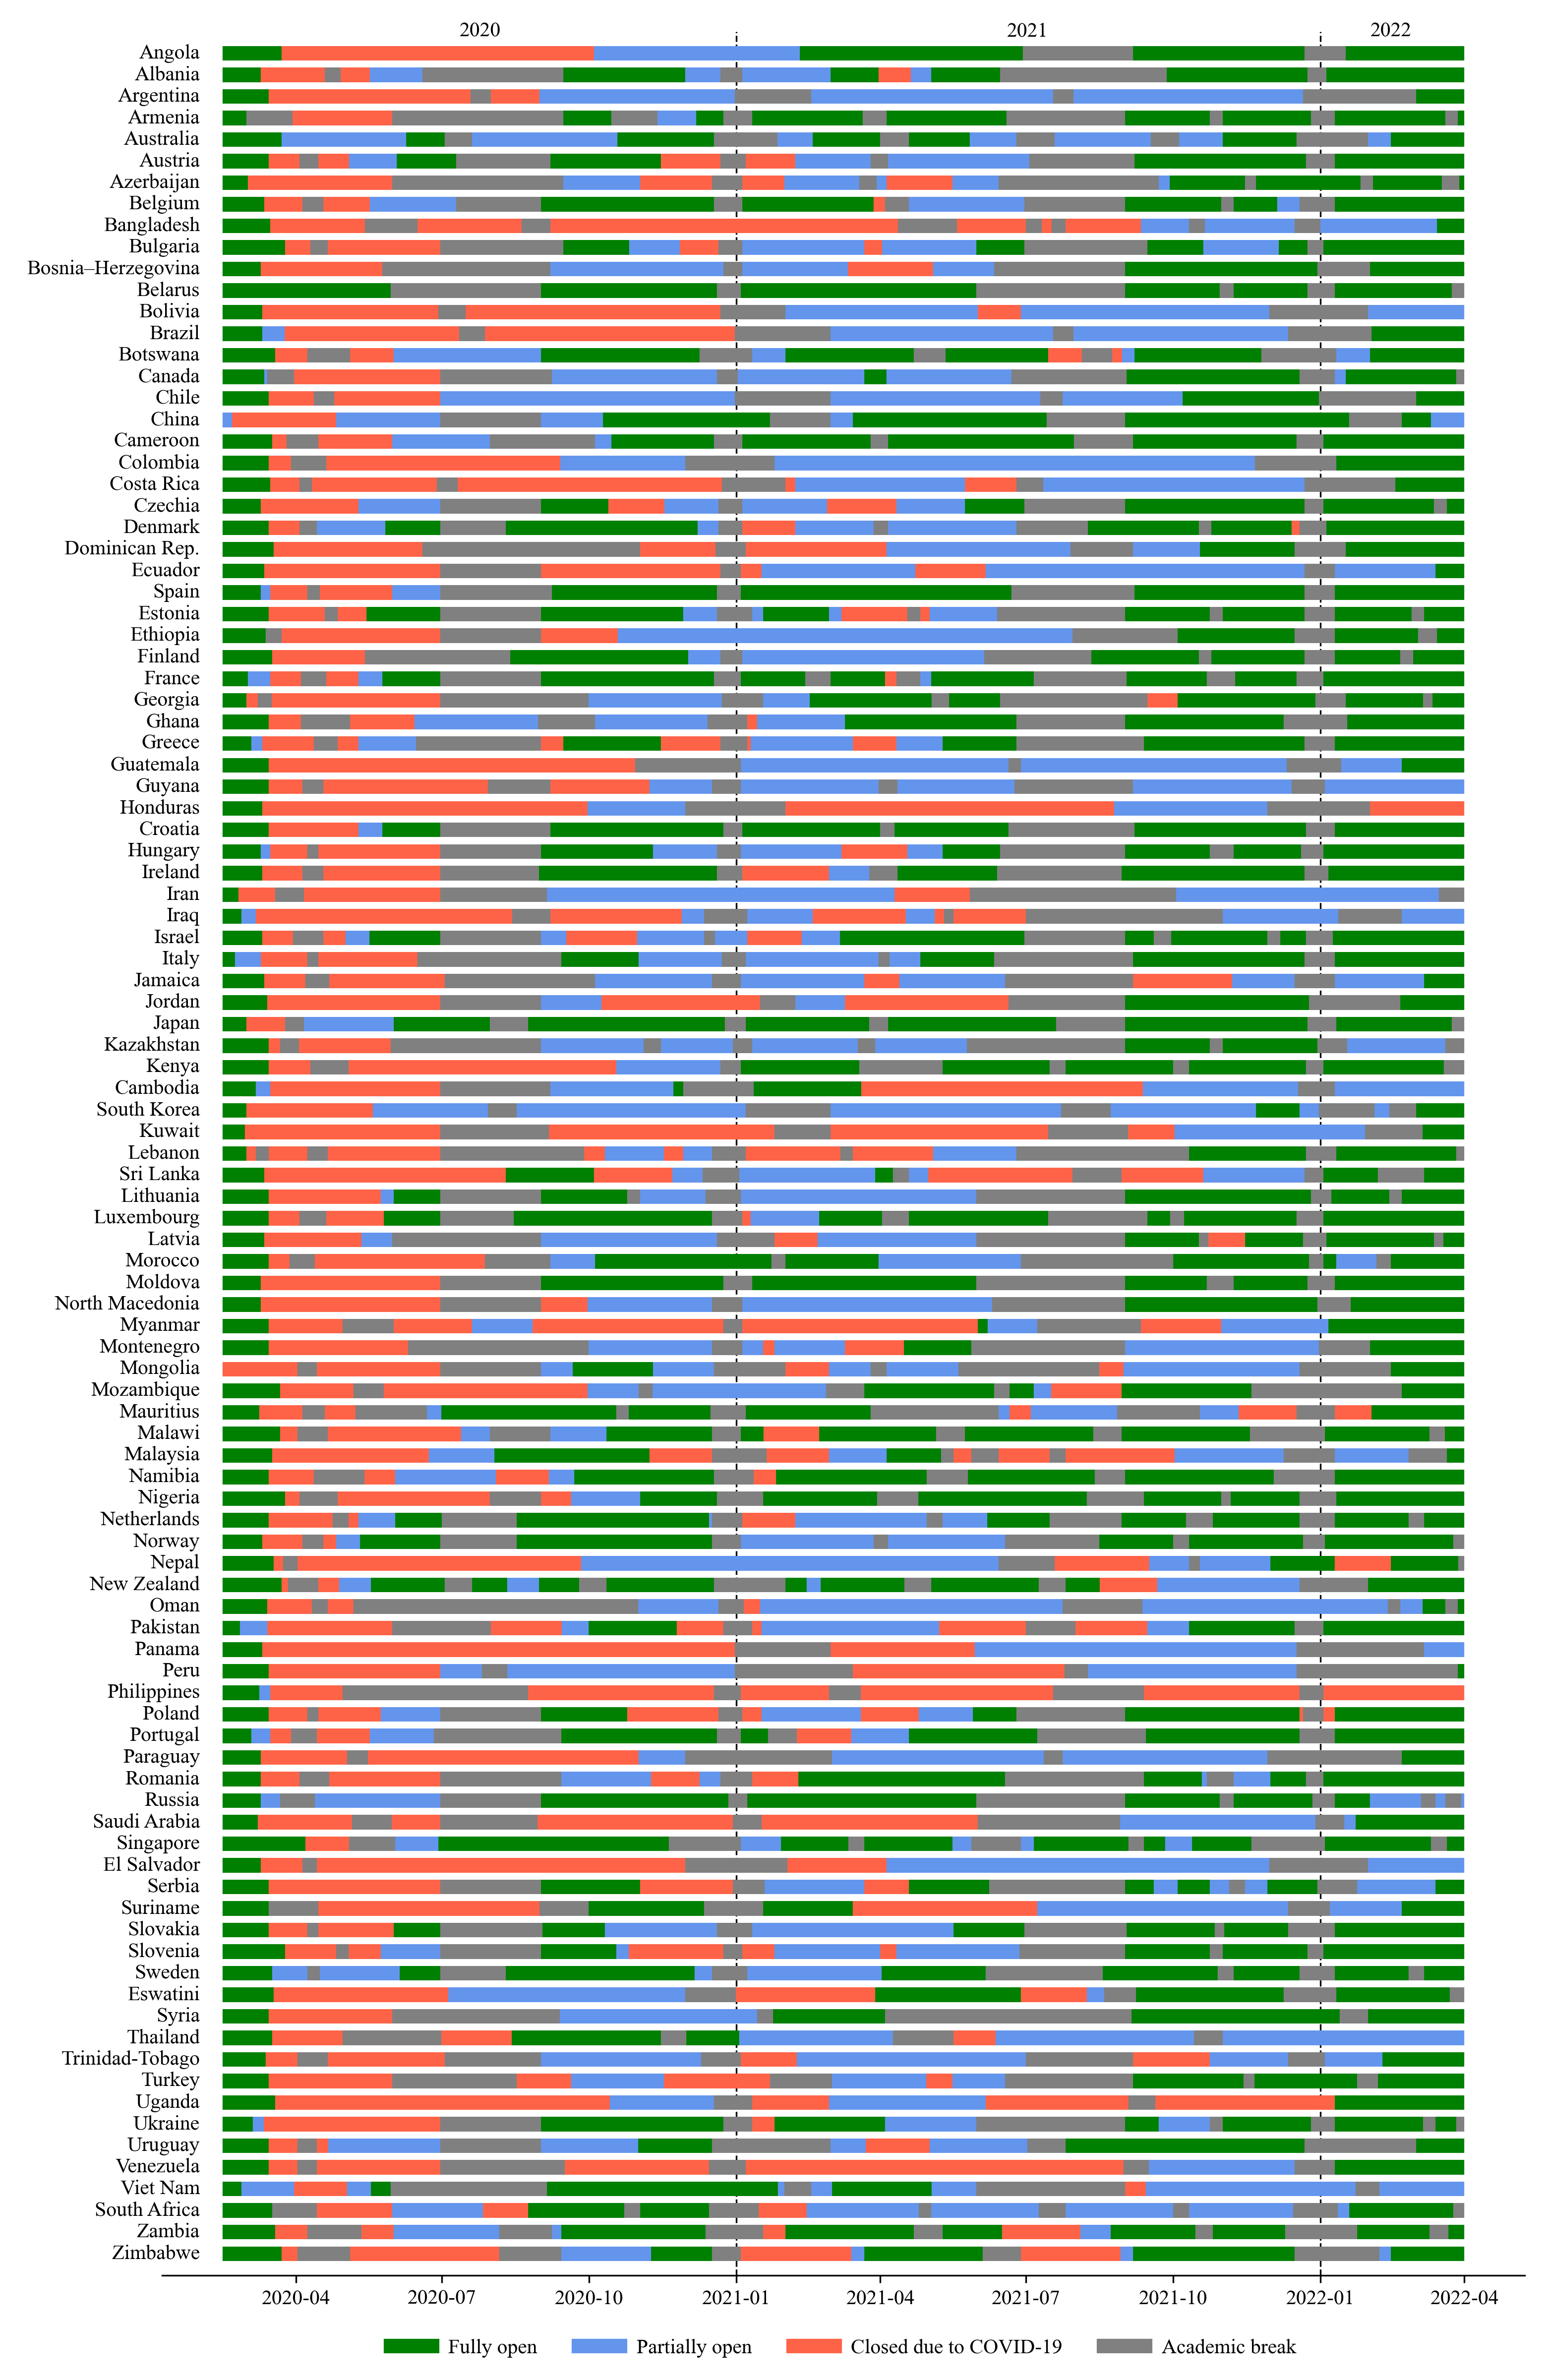
\includegraphics[width=0.73\textwidth]{../../tex_descriptions/projects/sm_covid/school_closures/unesco.png}
  \end{center}
  \caption{UNESCO data on school closures during the COVID-19 pandemic.
  } 
  \label{fig:unesco}
\end{figure}

\vspace{5pt}
\textbf{Dynamic mobility outside of schools and homes}

Changes to people's mobility in places other than schools and homes are modelled using Google Mobility data. We use the ``Workplace''
category of the Google data to scale the work-related matrix contribution $C_W$ to overall mixing over time, using the adjusting function
$w$. The ``other locations'' matrix $C_L$ is scaled through the adjusting function $l$ which is defined as the average of the Google mobility
indicators across the following Google categories: ``Retail and recreation'', ``Grocery and pharmacy'' and ``Transit stations''.

\vspace{5pt}
\textbf{Household contacts}

In the base case analysis, the contribution of household contacts to the overall mixing matrix is fixed over time 
(i.e. $h(t) = 1$ in Equation \ref{eq_mixing}). Although Google provides mobility 
estimates for residential contacts, the nature of these data is different from that of each of the other Google mobility 
types. They represent the time spent in that location, as opposed to other categories, which measure a change in total visitors 
rather than the duration. The daily frequency with which people attend their residence is likely to be close to one and we 
considered that household members likely have a daily opportunity for infection with each other household member regardless of
the background level of mobility. Therefore, we did not implement a function to scale the contribution of household contacts 
to the mixing matrix with time.

In a Sensitivity Analysis, we consider an alternative assumption where the effective contact rates within households are increased during
periods of school closure. In that case, the household component of the mixing matrix is modified by the following function:
$$ h(t) = 1 + 0.20(1 - s(t)) \quad ,$$ 
where $s$ is the function modifying school contacts as introduced in Section \ref{time_var_mixing}.

